%% Based on a TeXnicCenter-Template by Gyorgy SZEIDL.
%%%%%%%%%%%%%%%%%%%%%%%%%%%%%%%%%%%%%%%%%%%%%%%%%%%%%%%%%%%%%

%----------------------------------------------------------
%

%
%----------------------------------------------------------
% This is a sample document for the LaTeX Slides Class
% Class options
%       --  Body text point size (normalsize) is 27 (default)
%           and can not be adjusted to any other value.
%       --  Paper size:  letterpaper (8.5x11 inch, default)
%                        a4paper, a5paper, b5paper,
%                        legalpaper, executivepaper
%       --  Orientation (portrait is the default):
%                        landscape
%       --  Quality:     final(default), draft
%       --  Title page:  titlepage, notitlepage
%       --  Columns:     onecolumn (default), [twocolumn is not avalible]
%       --  Equation numbering (equation numbers on the right is the default)
%                        leqno (equation numbers on the left)
%       --  Displayed equations (centered is the default)
%                    fleqn (flush left)
%
%  \documentclass[a4paper,fleqn]{slides}
%
%  The slides are separated from each other by the slide
%  environment, see below:
%


\PassOptionsToPackage{table}{xcolor}
\documentclass[xcolor=dvipsnames]{beamer}
\usepackage[latin1]{inputenc}
\usepackage[T1]{fontenc}
\usepackage[ngerman]{babel}
\usepackage{amsmath}
\usepackage{amssymb,amsfonts,textcomp}
\usepackage{array}
\usepackage{hhline}
\usepackage{lmodern}
%\usepackage{epsfig}
\usepackage{graphics}
\usepackage{exscale} %Skalierung der Mathesymbole
\usepackage{ifthen}
\usepackage{epic,eepic}
\usepackage{color}
\usepackage{hyperref}
\usepackage[absolute,overlay]{textpos}
\usepackage{booktabs}
\usepackage{url}

\usetheme{PaloAlto}
\useinnertheme{rounded}
%\definecolor{tuc}{cmyk}
%\definecolor{tuc}{RGB}{0,90,70}
%\definecolor{tuc}{RGB}{23,118,101}%{40,128,255} %
\definecolor{tuc}{RGB}{255,255,9}
\usecolortheme[named=tuc]{structure}

%%% --------------------------------------------------------------
\setbeamercolor{title}{fg=black}
\setbeamercolor{title in sidebar}{fg=black}
\setbeamercolor{author in sidebar}{fg=black}
\setbeamercolor{subsection in sidebar}{fg=black}
\setbeamercolor{section in sidebar}{fg=black}
\setbeamercolor{frametitle}{fg=black}

\logo{
\includegraphics[width=1.5cm]{chch.png}}
\begin{document}
\title{\TeX tsatz im Alltag}
\author{Stefan Helmert}
\date{14.02.2014}
%\maketitle
% ----------------------------------------------------------------


\frame{\titlepage 
	\begin{textblock}{5}(11,10)
		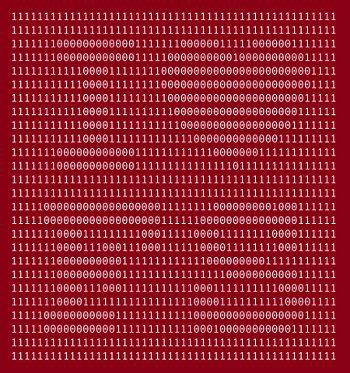
\includegraphics[width=3cm]{ILFSD.jpg}	
	\end{textblock}
}

\section[Textsatz]{Textsatz statt Textverarbeitung}
\frame
{
\textbf{\LaTeX\ -- Textsatz statt Textverarbeitung}
	\begin{itemize}
		\item sieht (hoffentlich) gut aus
		\item Bilder, Zeichnungen, Formeln, Inhalts- und Literaturverzeichnis
		\item Layout
		\item Flexibilit�t, Schnittstellen, Automatisierung
		\item Ausgabeformate
		\item Standard
		\item Community
		\item ohne Spezialsoftware
		\item stabil
		\item kompatibel
	\end{itemize}
	"`LaTeX was originally written in the early 1980s by Leslie Lamport at SRI International."' (\url{http://en.wikipedia.org/wiki/LaTeX})
}

\section{Editoren}
\frame
{
\textbf{Texteditor reicht}

\begin{itemize}
	\item vim
	\item Xemacs
	\item Notepad++
\end{itemize}

\textbf{besser \LaTeX -Editor}
\begin{itemize}
	\item \TeX niccenter
	\item \TeX Live
	\item i\TeX Mac2
\end{itemize}

\url{en.wikipedia.org/wiki/Comparison_of_TeX_editors}
}

\section{Compiler}
\frame
{
\textbf{Compiler}

Windows: \url{http://miktex.org/download}

Mac: \url{https://www.tug.org/mactex/}

Linux: \url{https://www.tug.org/texlive/}

}

\section{Briefe schreiben}
\frame
{
\textbf{Briefe}
\begin{itemize}
	\item Vorlage --  Anschrift, Datum, Betreff an richtiger Stelle
	\item automatisch aktuelles Datum
	\item Falzkanten
	\item Serienbrief
	\item Aufteilung in Dateien -- Textbl�cke
\end{itemize}
}

% ----------------------------------------------------------------

\end{document}
